\documentclass[pdflatex,sn-mathphys-num,iicol]{sn-jnl}

\usepackage{bookmark}
\usepackage{tabularx}
\usepackage{tikz}
\usetikzlibrary{shapes.geometric, shapes.misc, arrows.meta, positioning, calc}
\usepackage{graphicx}
\usepackage{amsmath,amssymb,amsfonts}
\usepackage{booktabs}

\raggedbottom

\begin{document}

\title[Evaluating CNN for Piano Chord Recognition]{Evaluating CNN for Piano Chord Recognition Under Acoustic Domain Shift}

\author*[1]{\fnm{Cikal} \sur{Gemintang Seya}}\email{cikalgemintangseya1@gmail.com}

\author[1]{\fnm{Jasman} \sur{Pardede}}\email{jasman@itenas.ac.id}

\affil*[1]{\orgdiv{Informatics}, \orgname{Institut Teknologi Nasional Bandung}, \orgaddress{\street{Neglasari}, \city{Bandung}, \postcode{40124}, \state{West Java}, \country{Indonesia}}}

\abstract{Automatic chord recognition from audio covers transcription, music education, and performance feedback. Classification models for it are normally trained and tested under one set of recording conditions. Different combinations of instrument, microphone, or room changes the recorded signal, and a single evaluation measured under a joint change does not say which factor is most impactful. This paper introduces 36-class piano chord datasets, consisting of 12 roots and three intervals (major, minor, diminished). We train a Convolutional Neural Network (CNN) on Constant-Q Transform (CQT) features from a Techno T-9890i digital keyboard and evaluate it without fine-tuning under a recording configuration shift, where the same keyboard is captured on three other microphones in different setups, then a keyboard shift, where a Yamaha PSR-S910 is captured on two of those same recording settings, and finally under evaluation-only overlays with ESC-50 noises, room impulse responses (RIR), and device impulse responses (DIR). The architecture is retrained ten times, five seeds on the full 7{,}200-clip training set (\texttt{orig}) and five after dropping silent and duplicated clips (\texttt{clean}). In-domain accuracy is 1.000 on every retrain. Out of domain, the keyboard gap is positive on 19 of 20 matched checkpoints and larger than the recording-setting drop on 17, overlay noise widens it, and a bank of 67 DIRs lowers accuracy by under 2 points, so convolving a microphone response does not reproduce a recorded microphone change. Seed-to-seed spread is large enough to move a Yamaha score by tens of points, so we report every seed.}

\keywords{automatic chord recognition, Constant-Q Transform, Convolutional Neural Network, domain shift, ablation, seed variance}

\maketitle

\section{Introduction}\label{sec_introduction}

Recognizing musical chords directly from raw audio is a foundational task in music information retrieval (MIR), underpinning automatic transcription, interactive music education, and real-time performance feedback \cite{Kusaka2024,zbaltan2024}. Unlike symbolic recognition, it must contend with sound production, since a chord played on one instrument, in one room, captured by one microphone does not produce the waveform of the same chord on a different set of recording configuration \cite{Kusaka2024}.

That mismatch is acoustic domain shift, a change in the recorded signal rather than a claim that the instruments are acoustic pianos, and at least three factors drive it. Piano variation is the first, where another instrument's voicing displaces chord vectors in feature space. Environmental shift is the second, where ambient noise and room acoustics absent from training move the scene. Recording-setting shift is the third, where a different microphone and placement change the captured spectrum \cite{Kusaka2024}. A classifier that latched onto a condition-specific cue instead of the interval structure pays for it out of domain \cite{Geirhos2020}. A joint shift matches deployment, but one number hides the cause, because a change of microphone, a change of instrument, and a noisy room are three different problems. Ranking the factors needs independently recorded datasets for each, plus a controlled synthetic overlay for the environment.

Time-frequency matrices classified with convolutional architectures dominate audio recognition \cite{Zaman2023}, and chord recognition has used them since the first frame-level CNN acoustic models \cite{Korzeniowski_2016}. The Constant-Q Transform (CQT) suits piano audio because, unlike the Short-Time Fourier Transform's linear bins, its bins are logarithmically spaced at a constant quality factor and align with semitones \cite{Lacoste2007}, so a transposition is a vertical shift and harmonic intervals keep a consistent shape \cite{Li2021}. Li \cite{Li2021} reported 84.2\% accuracy for CQT chord recognition against 75.3\% for STFT and 80.8\% for CENS chromagrams under one CNN. We keep CQT as the input. The 36 chord classes formed by 12 chromatic roots and 3 qualities demand fine-grained discrimination, since major and minor triads differ by a semitone in the third and diminished triads differ by a further semitone in the fifth \cite{Harte2010}. %Convolutional kernels respond to small time-frequency neighborhoods \cite{Purwono2022}, so local interval geometry can in principle survive the envelope shift a new microphone or piano voice imposes.

Edwards et al.\ \cite{Edwards2024} run the closest controlled piano out-of-domain study, though on note-level transcription rather than chords. They replay MAESTRO MIDI on a Yamaha Disklavier in a studio, evaluate on MAPS, and degrade test audio with noise, EQ, pitch shift, and reverb. A studio-only model overfits that environment, and train-time mixing then recovers 88.4 MAPS note-onset F1 with no MAPS training audio. Kusaka and Maezawa \cite{Kusaka2024} use a related approach for mobile transcription. Both treat augmentation as a training intervention, whereas we keep the opposite protocol, a clean-trained CQT--CNN with recorded and synthetic shifts only at evaluation, so the drop each factor causes is visible before anyone mixes the training set. Their pianos are acoustic and ours are digital, so the keyboard factor here is a change of piano sound, not in terms of physical acoustic piano.

Chord papers still grow the vocabulary or swap in conformers \cite{Akram2025}, test in-domain, and patch out-of-domain conditions with synthetic audio \cite{Majchrzak2025,Ostermann2023}. Isolated piano chords lack a factorized reading of a CQT--CNN that also asks whether a training-set defect changes the ranking. Sixteen digital-silence clips, 8\% of $C$ diminished, and twelve exact CQT duplicates in $A\sharp$ major sit in the Techno training set. In-domain accuracy saturates at 1.00 and cannot answer that question. Since a single-run benchmark hides this kind of spread \cite{Bouthillier2021}, we retrain the architecture ten times, five seeds on the full set (\texttt{orig}) and five after those 28 clips are dropped (\texttt{clean}), and report every seed on every held-out condition.

This paper makes four contributions.
\begin{enumerate}
\item A corpus recorded to separate the factors. A Techno T-9890i training set with five held-out datasets: three recording-setting-shift datasets on that same keyboard, one of which (\texttt{vivo}) has no keyboard counterpart, and two Yamaha PSR-S910 keyboard-shift datasets captured on recording settings already used for the recording-setting tests.
\item A shared representation and a repeated retrain. One CQT feature format ($216\times188\times1$) into a compact CNN, retrained under two training-set configurations and five seeds on a single pinned GPU with deterministic kernels.
\item A frozen-weight evaluation protocol. Recording-setting change is tested apart from keyboard change with no fine-tuning, and eval-only noise, room, and microphone overlays are then applied on top, every seed reported.
\item A per-seed ranking of the factors. The recorded factors are ordered against each other and against the synthetic overlays, including a Techno-test-split control that measures the overlays without a recorded device or keyboard change. The ablation of 28 defective training clips asks whether a data-quality fix changes that order.
\end{enumerate}

\section{Methodology}\label{sec_methodology}

Fig.~\ref{fig_methodology} shows the pipeline, running from dataset acquisition through CQT extraction, the \texttt{orig}/\texttt{clean} $\times$ 5-seed CNN retrain, recorded out-of-domain evaluation, and eval-only overlays. The software stack is Python 3.10, TensorFlow 2.15, scikit-learn 1.7.2, Librosa 0.11.0, NumPy 1.26.4, and Matplotlib 3.10.8.

\begin{figure}[htbp]
  \centering
  \resizebox{0.92\columnwidth}{!}{%
  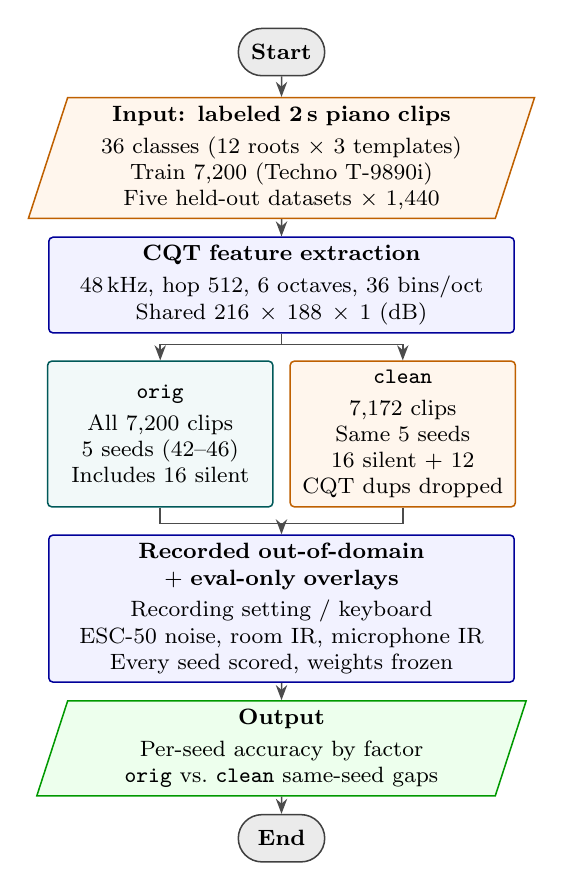
\begin{tikzpicture}[
    node distance=0.16cm and 0.10cm,
    >={Stealth},
    font=\footnotesize,
    base/.style={draw, align=center, minimum height=0.52cm, line width=0.55pt, inner sep=3pt},
    terminal/.style={base, shape=rounded rectangle, rounded rectangle arc length=180, draw=black!75, fill=black!8, minimum height=0.60cm, minimum width=1.8cm, inner xsep=10pt, inner ysep=2pt, font=\footnotesize\bfseries},
    process/.style={base, rectangle, rounded corners=1.5pt, draw=blue!60!black, fill=blue!5, text width=5.7cm},
    orig/.style={base, rectangle, rounded corners=1.5pt, draw=teal!70!black, fill=teal!5, text width=2.65cm, minimum height=1.85cm},
    clean/.style={base, rectangle, rounded corners=1.5pt, draw=orange!75!black, fill=orange!7, text width=2.65cm, minimum height=1.85cm},
    io/.style={base, trapezium, trapezium left angle=72, trapezium right angle=108, trapezium stretches body=true, draw=orange!75!black, fill=orange!7, text width=5.15cm, inner xsep=4pt},
    result/.style={base, trapezium, trapezium left angle=72, trapezium right angle=108, trapezium stretches body=true, draw=green!60!black, fill=green!7, text width=5.15cm, inner xsep=4pt},
    arrow/.style={->, line width=0.55pt, black!70}
  ]
    \node[terminal] (start) {Start};
    \node[io, below=0.26cm of start] (in1)
    {\textbf{Input: labeled 2\,s piano clips}\\[2pt]
     36 classes (12 roots $\times$ 3 templates)\\
     Train 7{,}200 (Techno T-9890i)\\
     Five held-out datasets $\times$ 1{,}440};
    \node[process, below=0.22cm of in1] (p2)
    {\textbf{CQT feature extraction}\\[2pt]
     48\,kHz, hop 512, 6 octaves, 36 bins/oct\\
     Shared $216 \times 188 \times 1$ (dB)};
    \node[orig, below left=0.34cm and 0.10cm of p2.south, anchor=north east] (o1)
    {\textbf{\texttt{orig}}\\[2pt]
     All 7{,}200 clips\\
     5 seeds (42--46)\\
     Includes 16 silent};
    \node[clean, below right=0.34cm and 0.10cm of p2.south, anchor=north west] (c1)
    {\textbf{\texttt{clean}}\\[2pt]
     7{,}172 clips\\
     Same 5 seeds\\
     16 silent $+$ 12 CQT dups dropped};
    \node[process, below=0.34cm of $(o1.south)!0.5!(c1.south)$, anchor=north] (p5)
    {\textbf{Recorded out-of-domain $+$ eval-only overlays}\\[2pt]
     Recording setting / keyboard\\
     ESC-50 noise, room IR, microphone IR\\
     Every seed scored, weights frozen};
    \node[result, below=0.22cm of p5] (out)
    {\textbf{Output}\\[2pt]
     Per-seed accuracy by factor\\
     \texttt{orig} vs.\ \texttt{clean} same-seed gaps};
    \node[terminal, below=0.22cm of out] (endn) {End};
    \draw[arrow] (start) -- (in1);
    \draw[arrow] (in1) -- (p2);
    \draw[arrow] (p2.south) -- ++(0,-0.14) -| (o1.north);
    \draw[arrow] (p2.south) -- ++(0,-0.14) -| (c1.north);
    \coordinate (merge) at ($(p5.north)+(0,0.14)$);
    \draw[line width=0.55pt, black!70] (o1.south) |- (merge);
    \draw[line width=0.55pt, black!70] (c1.south) |- (merge);
    \draw[arrow] (merge) -- (p5.north);
    \draw[arrow] (p5) -- (out);
    \draw[arrow] (out) -- (endn);
  \end{tikzpicture}%
  }
  \caption{Experimental pipeline. Shared CQT features feed two training-set variants $\times$ five seeds. Eval-only overlays hit the five held-out datasets; CNN weights stay frozen after training.}
  \label{fig_methodology}
\end{figure}

\subsection{Two evaluation scenarios}\label{subsec_scenarios}

Scenario~1 (in-domain) holds instrument, environment, and recording setting fixed and asks whether the CQT space separates the 36 classes at all. Five-fold cross-validation on each training pool measures this, with a 20\% test fold, a 10\% validation slice of the remaining pool (70/10/20 overall), a fresh initialization, and a fixed per-fold seed. Each retrain below also reports its own held-out Techno test split.

Scenario~2 changes one factor at a time and tests each trained checkpoint with no fine-tuning. Three recording-setting-shift datasets keep the Techno T-9890i and change the microphone and its placement (ThinkPad P14s internal mic, Vivo Y27s, ROG Flow X13 internal mic). Laptop and phone capture paths commonly apply automatic gain control and noise suppression that neither device logs, so this factor bundles transducer, codec, and unrecorded processing rather than isolating a frequency response. Two keyboard-shift datasets swap the instrument to a Yamaha PSR-S910 while reusing the ThinkPad and Flow recording settings already measured on the Techno, so \texttt{thinkpad} versus \texttt{thinkpad-2} and \texttt{flow} versus \texttt{flow-2} differ by keyboard alone. \texttt{vivo} has no Yamaha counterpart. Table~\ref{tab_datasets} lists all six datasets, and eval-only overlays (Section~\ref{subsec_noise}) hit the five held-out ones.

\begin{table*}[t]
\caption{Recorded datasets. The CNN is trained on \texttt{training} and evaluated on every row. $^\dagger$\texttt{vivo} has no Yamaha counterpart.}\label{tab_datasets}
\begin{tabular*}{\textwidth}{@{\extracolsep{\fill}}lllll@{}}
\toprule
Dataset & $N$ & Primary shift & Instrument & Recording setting \\
\midrule
\texttt{training} & 7{,}200 & None (in-domain) & Techno T-9890i & Redmi Pad 2 \\
\texttt{thinkpad} & 1{,}440 & Recording setting & Techno T-9890i & ThinkPad P14s \\
\texttt{vivo} & 1{,}440 & Recording setting$^\dagger$ & Techno T-9890i & Vivo Y27s \\
\texttt{flow} & 1{,}440 & Recording setting & Techno T-9890i & ROG Flow X13 \\
\texttt{thinkpad-2} & 1{,}440 & Keyboard & Yamaha PSR-S910 & ThinkPad P14s \\
\texttt{flow-2} & 1{,}440 & Keyboard & Yamaha PSR-S910 & ROG Flow X13 \\
\bottomrule
\end{tabular*}
\end{table*}

\subsection{Dataset acquisition}\label{subsec_acquisition}

A web recorder sends simultaneous MIDI note-on events over USB and captures the microphone. Mechanised capture of this kind has been used before to build chord corpora without a human player \cite{Byambatsogt2020}. That removes manual playing errors and keeps each keyboard's loudspeaker, cabinet, and synthesis. Every dataset uses the same trigger list and voicing, so class identity does not change with the acoustic condition. Notes are sent at one fixed velocity with no modulation and no pitch bend, so every take shares the same attack and playing dynamics.

Each of the 36 classes is a three-note piano sound, one of 12 roots (C, C$\sharp$, \ldots, B) crossed with one of three interval templates (major $+4,+3$; minor $+3,+4$; diminished $+3,+3$ semitones). A semitone occupies three CQT bins. Figures write \emph{C maj} and \emph{E dim}. All takes sit in the fourth octave, inside C1--C7 (32.70--2{,}093\,Hz). The diminished interval packs its three notes closer together than major or minor. The Techno T-9890i is a consumer arranger keyboard and the Yamaha PSR-S910 a workstation arranger, both are digital instruments put on a grand piano preset with a different piano sound.

The training set holds 200 samples per class, 7{,}200 total, from the Techno on an Acoustic Grand preset into a Redmi Pad 2 microphone, stored in Opus format at 48{,}000\,Hz, mono channel, with attack delays of 0--150\,ms approximating keystroke asynchrony for variety. Sixteen of those clips, 8\% of $C$ diminished and a recorder fault, are digital silence. Twelve further $A\sharp$ major takes are exact CQT duplicates (six pairs). Section~\ref{subsec_ablation} trains with the full set and after those 28 clips are dropped. Each held-out dataset holds 40 takes per class, 1{,}440 in all, written as 16-bit PCM WAV at 48{,}000\,Hz, with \texttt{vivo} mono and the four laptop sets stereo. No evaluation clip enters training, validation, early stopping, or hyperparameter choice.

\subsection{CQT feature extraction}\label{subsec_cqt}

We compute CQT with \texttt{librosa.cqt()}. Each bin $f_k$ has constant quality
\begin{equation}
Q = \frac{f_k}{f_{k+1} - f_k} = \frac{1}{2^{1/B} - 1}
\label{eq_cqt}
\end{equation}
where $B$ is bins per octave \cite{Li2021,Lacoste2007}. Logarithmic spacing lines bins up with semitones, so a major third is the same bin distance on every root \cite{Harte2010}.

Analysis runs at 48\,kHz with hop 512, a Hann window, and 6 octaves at 36 bins per octave, covering C1 (32.70\,Hz) to C7 (2{,}093\,Hz) in 216 bins. Loading resamples every clip to that rate and mixes stereo channels down to mono. Three bins per semitone resolve the three interval templates. Each clip is truncated to a fixed 2.0\,s, so Equation~\ref{eq_frames} gives $2.0\times 48000/512=187.5$, and the stored CQT rounds up to 188 frames with shape $216 \times 188 \times 1$. Magnitudes are converted to decibels relative to each clip's own loudest bin, which therefore sits at 0\,dB. Training, every recorded dataset, and every overlay share these parameters.

\begin{equation}
\text{frames} = \frac{\text{duration} \times \text{sample rate}}{\text{hop size}}
\label{eq_frames}
\end{equation}

\begin{figure}[htbp]
\centering
\includegraphics[width=\columnwidth]{fig-cqt-train.png}
\caption{Training CQT of C maj ($+4,+3$) and C min ($+3,+4$): same root, one-semitone gap in the middle note. Frequency in Hz.}
\label{fig_cqt}
\end{figure}

\subsection{CNN architecture and training}\label{subsec_cnn}

The CNN follows Wolf-Monheim \cite{Wolf-Monheim2025}, originally designed for environmental sound classification on ESC-50. Its compact four-block convolutional structure without recurrent layers or attention suits fixed-window classification from static spectrograms. Surveys of deep audio classification separate convolutional, recurrent, and attention-based families largely by how much temporal context they model \cite{Zaman2023}.

Table~\ref{tab_cnn_arch} lists layers. The input batch-normalization layer runs on the frequency axis, fitting one scale and shift per CQT bin to the Techno training distribution and applying that fixed 216-parameter transform to every clip at inference. The four Conv2D--MaxPooling2D blocks build a hierarchy that moves from 64 filters for low-level spectral texture to 128 for mid-level interval patterns and then two blocks of 256 for chord-quality abstractions. A single $3\times3$ kernel spans one semitone at 3 bins per semitone, narrower than the maj/min/dim contrast, so quality discrimination accumulates across blocks as pooling widens the effective receptive field \cite{Purwono2022}. Flatten feeds 36{,}608 units into a 256-unit dense layer, about 9.4\,M of the model's parameters, and that layer reads absolute time-frequency position. Apart from dropout at the head the design carries no regularization, with no weight decay and no train-time augmentation.

\begin{table}[t]
\caption{CNN architecture specification}\label{tab_cnn_arch}
\begin{tabularx}{\columnwidth}{@{}lXl@{}}
\toprule
Layer & Output shape & Notes \\
\midrule
BatchNorm & $216{\times}188{\times}1$ & Per frequency bin \\
Conv2D & $216{\times}188{\times}64$ & $3{\times}3$, ReLU, same \\
MaxPool & $108{\times}94{\times}64$ & $2{\times}2$, stride 2 \\
Conv2D & $108{\times}94{\times}128$ & $3{\times}3$, ReLU, same \\
MaxPool & $54{\times}47{\times}128$ & $2{\times}2$, stride 2 \\
Conv2D & $54{\times}47{\times}256$ & $3{\times}3$, ReLU, same \\
MaxPool & $27{\times}23{\times}256$ & $2{\times}2$, stride 2 \\
Conv2D & $27{\times}23{\times}256$ & $3{\times}3$, ReLU, same \\
MaxPool & $13{\times}11{\times}256$ & $2{\times}2$, stride 2 \\
Flatten & 36{,}608 & --- \\
Dense & 256 & ReLU \\
Dropout & 256 & rate 0.5 \\
Dense & 36 & Softmax \\
\bottomrule
\end{tabularx}
\end{table}

Training follows Table~\ref{tab_cnn_train}. A stratified 10\% test split is drawn first, then a stratified $1/9$ of the remainder becomes validation, giving 80/10/10 of the pool ($160/20/20$ per class on \texttt{orig}). The seed sets both splits, the weight initialization, and the Python, NumPy, and TensorFlow global RNGs, so a seed here indexes a bundle of split and initialization rather than initialization alone. \texttt{ReduceLROnPlateau} multiplies the learning rate by 0.1 after 2 stagnant validation-loss epochs, \texttt{EarlyStopping} stops after 6 and restores the best-validation-loss weights \cite{Wolf-Monheim2025}. Training runs for a maximum of 50 epochs and each of the ten retrains ran on its own, on the same GPU and with deterministic kernels, so the seed-to-seed spread reported below is not hardware variation.

\begin{table}[t]
\caption{CNN training configuration}\label{tab_cnn_train}
\begin{tabular}{@{}ll@{}}
\toprule
Parameter & Value \\
\midrule
Seeds & 42, 43, 44, 45, 46 \\
Train / Val / Test split & 80\% / 10\% / 10\% \\
Batch size & 32 \\
Initial learning rate & 0.001 \\
Optimizer & Adam \\
Weight initialization & Glorot uniform \\
Loss & Categorical cross-entropy \\
Max epochs & 50 \\
EarlyStopping & patience 6, restore best \\
ReduceLROnPlateau & factor 0.1, patience 2 \\
\bottomrule
\end{tabular}
\end{table}

\subsection{Training-set ablation}\label{subsec_ablation}

Two training configurations share Table~\ref{tab_cnn_arch} and Table~\ref{tab_cnn_train}. \texttt{orig} uses all 7{,}200 clips. \texttt{clean} drops the sixteen silent $C$ diminished takes and one member of each of the twelve exact $A\sharp$ major CQT pairs (7{,}172 remaining) and changes no hyperparameter. Each is retrained from seeds 42--46, producing ten checkpoints.

The seed generates the split from whichever pool it is handed, so \texttt{orig} seed 42 and \texttt{clean} seed 42 draw different train/validation/test partitions as well as different initializations, and the seed value is the only quantity they share. Same-seed comparisons below therefore measure dropping the clips and redrawing the split together. Deleting the defective clips from inside a fixed partition would separate the two, but that run is not in this report.

\subsection{Evaluation-only overlays}\label{subsec_noise}

Three overlays hit the already out-of-domain datasets without retraining, applied to all ten checkpoints with overlay probability 1, a fixed draw seed, and no write-back into training. The same three overlays are also applied to each checkpoint's Techno test split (720 clips on \texttt{orig}, 718 on \texttt{clean}), so the overlay drop can be read with no recorded device or keyboard change.

\emph{Noise.} 400 ESC-50 clips over 10 interior and domestic classes \cite{Piczak2015} become CQT matrices under the same hop and binning as the chord features. Each chord clip is added to one noise matrix, started at a random point in the noise clip and scaled so that the signal-to-noise ratio over the whole clip matches a target drawn uniformly from $[10,25]$\,dB.
%\begin{equation}
%Y = \sqrt{X^{2} + \alpha^{2} N^{2}}, \quad
%\alpha^{2} = \frac{\overline{X^{2}}}{\overline{N^{2}}\,10^{\,\mathrm{SNR}/10}} ,
%\label{eq_mix}
%\end{equation}
The mixing is done on the CQT rather than on the waveform, which leaves out how the two sounds would interfere and how a microphone would capture them together, so this is a controlled interior overlay rather than a claim that ESC-50 matches a recorded environment.

\emph{Room and device impulse responses.} These convolve the evaluation waveform before CQT extraction, one response drawn per clip. The room impulse response (RIR) bank holds 174 indoor responses from the IR Survey \cite{Traer2016} with bathrooms and outdoor spaces removed. The device impulse response (DIR) bank holds 67 responses from micIRP\footnote{https://micirp.blogspot.com/}, a set of measured responses from old studio microphones, Kusaka and Maezawa use at model training \cite{Kusaka2024}. Both banks are resampled to 48\,kHz, leading-silence trimmed, and the wet waveform is peak-normalized.

\subsection{Evaluation metrics}\label{subsec_metrics}

Accuracy is the fraction of clips with the correct label, and macro precision, recall, and F1 are unweighted means of the performance over the 36 classes. Tables report accuracy per seed. A \emph{keyboard gap} is how much accuracy one checkpoint loses when the keyboard changes and the recording setting stays fixed, read from \texttt{thinkpad} against \texttt{thinkpad-2} and from \texttt{flow} against \texttt{flow-2}. An \emph{overlay drop} is how much accuracy the same checkpoint loses on a dataset once an overlay is applied to it, and on the Techno test split it is read the same way against the unmodified split. Both are stated in accuracy points. Differences smaller than roughly 3 points between two 1{,}440-clip cells are too small for datasets of this size to resolve.

\section{Results}\label{sec_results}

\subsection{In-domain performance}\label{subsec_res_indomain}

Every clip becomes a $216 \times 188$ CQT dB matrix, and Fig.~\ref{fig_cqt} shows C maj and C min from the training set, the same root but one semitone apart in the middle note. Under Scenario~1 the CNN scores 0.9999 mean accuracy on five-fold cross-validation of each pool (one miss on \texttt{orig} fold 0 and one on \texttt{clean} fold 2, with the other eight folds at 1.000). On the held-out Techno test split of the ten retrains every seed reaches 1.000.

That saturation says less than it appears to. The 200 takes of a class share one keyboard, one preset, one fourth-octave voicing, and one MIDI trigger list, differing only by an attack delay of 0--150\,ms, so a random split places near-copies of each test clip in the training partition. In-domain 1.00 is close to a memorization check, and the 5-fold run measures the same near-degeneracy a second time. What this paper can answer is how far that memorizer transfers, which is Scenario~2.

\subsection{Recorded out-of-domain accuracy}\label{subsec_res_recorded}

Table~\ref{tab_seeds} lists accuracy for each seed, grouped by recording setting. Recording-setting means are 0.975 / 0.915 / 0.953 on \texttt{orig} and 0.984 / 0.877 / 0.938 on \texttt{clean} for \texttt{thinkpad}, \texttt{vivo}, and \texttt{flow}. The keyboard means sit lower, 0.799 and 0.812 on \texttt{orig} against 0.865 and 0.874 on \texttt{clean}. No seed repeats the Yamaha collapse seen in an earlier 7{,}184-clip \texttt{clean} run. The weakest Yamaha cells here are \texttt{orig} seed 43 at 0.689 / 0.721 and \texttt{clean} seed 42 at 0.738 / 0.711, while \texttt{clean} seed 44 holds 0.955 / 0.965. Same-seed \texttt{orig} versus \texttt{clean} comparisons still mix the dropped clips with a redrawn split (Section~\ref{subsec_ablation}).

\begin{table*}[t]
\caption{Out-of-domain accuracy by seed and recording setting, recorded (top) and under eval-only ESC-50 interior noise (bottom). Gap is Techno minus Yamaha on the same checkpoint, in accuracy points computed before rounding. \texttt{orig} keeps all 7{,}200 clips, \texttt{clean} drops 28 defective ones. \texttt{vivo} has no Yamaha pair. $^\dagger$Gap inside the $\pm3$-point resolution.}\label{tab_seeds}
\setlength{\tabcolsep}{3.5pt}
\begin{tabular*}{\textwidth}{@{\extracolsep{\fill}}llccccccc@{}}
\toprule
& & \multicolumn{3}{c}{ThinkPad} & \multicolumn{3}{c}{Flow} & Vivo \\
\cmidrule(lr){3-5} \cmidrule(lr){6-8}
Variant & Seed & Techno & Yamaha & Gap & Techno & Yamaha & Gap & Techno \\
\midrule
\multicolumn{9}{@{}l}{\textit{Recorded}} \\
\texttt{orig} & 42 & 0.995 & 0.858 & 13.7 & 0.949 & 0.854 & 9.4 & 0.898 \\
\texttt{orig} & 43 & 0.935 & 0.689 & 24.6 & 0.836 & 0.721 & 11.5 & 0.797 \\
\texttt{orig} & 44 & 0.972 & 0.778 & 19.3 & 0.986 & 0.791 & 19.5 & 0.957 \\
\texttt{orig} & 45 & 0.979 & 0.761 & 21.8 & 0.998 & 0.772 & 22.6 & 0.960 \\
\texttt{orig} & 46 & 0.995 & 0.907 & 8.8 & 0.998 & 0.924 & 7.4 & 0.965 \\
\textbf{\texttt{orig}} & \textbf{Mean} & \textbf{0.975} & \textbf{0.799} & \textbf{17.6} & \textbf{0.953} & \textbf{0.812} & \textbf{14.1} & \textbf{0.915} \\
\texttt{clean} & 42 & 0.962 & 0.738 & 22.4 & 0.829 & 0.711 & 11.8 & 0.670 \\
\texttt{clean} & 43 & 0.960 & 0.878 & 8.3 & 0.894 & 0.896 & $-0.1^\dagger$ & 0.792 \\
\texttt{clean} & 44 & 1.000 & 0.955 & 4.5 & 0.996 & 0.965 & 3.1 & 0.990 \\
\texttt{clean} & 45 & 0.999 & 0.858 & 14.0 & 0.982 & 0.882 & 10.0 & 0.935 \\
\texttt{clean} & 46 & 0.999 & 0.895 & 10.3 & 0.991 & 0.917 & 7.4 & 0.994 \\
\textbf{\texttt{clean}} & \textbf{Mean} & \textbf{0.984} & \textbf{0.865} & \textbf{11.9} & \textbf{0.938} & \textbf{0.874} & \textbf{6.4} & \textbf{0.877} \\
\midrule
\multicolumn{9}{@{}l}{\textit{Eval-only ESC-50 noise}} \\
\texttt{orig} & 42 & 0.824 & 0.648 & 17.6 & 0.797 & 0.658 & 13.8 & 0.760 \\
\texttt{orig} & 43 & 0.823 & 0.483 & 34.0 & 0.733 & 0.517 & 21.5 & 0.698 \\
\texttt{orig} & 44 & 0.838 & 0.501 & 33.7 & 0.865 & 0.533 & 33.3 & 0.817 \\
\texttt{orig} & 45 & 0.890 & 0.655 & 23.5 & 0.929 & 0.691 & 23.8 & 0.897 \\
\texttt{orig} & 46 & 0.953 & 0.837 & 11.6 & 0.954 & 0.841 & 11.3 & 0.893 \\
\textbf{\texttt{orig}} & \textbf{Mean} & \textbf{0.866} & \textbf{0.625} & \textbf{24.1} & \textbf{0.856} & \textbf{0.648} & \textbf{20.8} & \textbf{0.813} \\
\texttt{clean} & 42 & 0.823 & 0.640 & 18.3 & 0.678 & 0.624 & 5.4 & 0.576 \\
\texttt{clean} & 43 & 0.846 & 0.735 & 11.1 & 0.783 & 0.737 & 4.7 & 0.675 \\
\texttt{clean} & 44 & 0.941 & 0.828 & 11.3 & 0.931 & 0.855 & 7.6 & 0.897 \\
\texttt{clean} & 45 & 0.925 & 0.735 & 19.0 & 0.906 & 0.753 & 15.3 & 0.833 \\
\texttt{clean} & 46 & 0.960 & 0.830 & 13.1 & 0.940 & 0.840 & 9.9 & 0.920 \\
\textbf{\texttt{clean}} & \textbf{Mean} & \textbf{0.899} & \textbf{0.754} & \textbf{14.5} & \textbf{0.848} & \textbf{0.762} & \textbf{8.6} & \textbf{0.780} \\
\bottomrule
\end{tabular*}
\end{table*}

\begin{figure*}[t]
\centering
\includegraphics[width=\textwidth]{fig-factors-overlays.pdf}
\caption{Per-checkpoint view of the results Table~\ref{tab_seeds} tabulates.
\textbf{(A)}~the twenty matched comparisons, keyboard gap against recording-setting drop on the same checkpoint. Points above the dashed line are comparisons where the keyboard is the larger factor; the three below it are all Flow.
\textbf{(B)}~mean accuracy removed by each eval-only overlay, with whiskers spanning the smallest and largest checkpoint--dataset cell. The Techno test split carries no recorded device or keyboard change.}
\label{fig_factors}
\end{figure*}

\subsection{Ranking the recorded factors}\label{subsec_res_factors}

Table~\ref{tab_seeds} isolates the keyboard with the two matched-pair gaps. Nineteen of the twenty checkpoint--pair combinations lose accuracy when the keyboard changes and the recording setting does not. The remaining cell, \texttt{clean} seed 43 on Flow, is $-0.1$ points and sits inside the resolution limit. On \texttt{orig} the ThinkPad gap runs from 8.8 to 24.6 points, and on \texttt{clean} from 4.5 to 22.4.

Ranking the two recorded factors against each other needs a common baseline. Reading the recording-setting drop as $1.000$ minus the Techno out-of-domain accuracy, and the keyboard drop as the matched gap on the same checkpoint, the keyboard is the larger factor on 17 of the 20 comparisons, which is panel A of Fig.~\ref{fig_factors}. All three exceptions fall on the Flow pair, where an unusually weak Techno baseline makes the recording-setting drop the larger of the two. Averaged over seeds and the three Techno sets, the recording setting lowers accuracy by 5.2 points on \texttt{orig} and 6.7 on \texttt{clean}, against mean keyboard gaps of 14.1--17.6 and 6.4--11.9.

\subsection{Where the keyboard error lands}\label{subsec_res_quality}

Averaged over the five seeds, the three qualities separate under keyboard shift. On \texttt{orig} the recall of major, minor, and diminished triads is 0.986 / 0.975 / 0.964 on \texttt{thinkpad} against 0.844 / 0.808 / 0.745 on \texttt{thinkpad-2}, and 0.980 / 0.947 / 0.934 on \texttt{flow} against 0.838 / 0.831 / 0.768 on \texttt{flow-2}. \texttt{clean} keeps the same order with a smaller drop, diminished falling to 0.802 and 0.828 on the two Yamaha sets. The $+3,+3$ template packs its notes closest together, and it is the first quality the model loses when the instrument changes. On \texttt{vivo} it already sits at 0.865 (\texttt{orig}) and 0.812 (\texttt{clean}) against 0.978 and 0.910 for major.

\subsection{Eval-only overlays}\label{subsec_res_noise}

The lower half of Table~\ref{tab_seeds} lists accuracy after ESC-50 interior noise is mixed into every evaluation clip, and the room and microphone banks were applied to the same frozen checkpoints. Noise lowers accuracy on all 50 dataset--seed cells of both variants. On \texttt{orig} the mean drop is 10.3 points on the three Techno sets and 16.9 on the two Yamaha sets, and on \texttt{clean} those figures are 9.1 and 11.2. Keyboard shift plus noise is the worst condition in the study, with Yamaha noise means of 0.625 / 0.648 on \texttt{orig} and 0.754 / 0.762 on \texttt{clean}, so noise stretches the ordering in the upper half of Table~\ref{tab_seeds} rather than changing it.

Fig.~\ref{fig_factors} panel B collects all three overlays. Indoor room impulse responses drop accuracy by 6.8 (\texttt{orig}) and 6.5 (\texttt{clean}) points on the Techno sets, less than noise, and by 7.2 / 8.8 on Yamaha. The 67-response DIR bank drops accuracy by 1.4 points on \texttt{orig} and 1.2 on \texttt{clean}, inside the resolution limit, while a recorded change of microphone and recording setup drops it by 5.2--6.7 points on the same checkpoints.

On each checkpoint's Techno test split the same overlays drop accuracy by 6.9 / 2.2 / 0.9 points (\texttt{orig}) and 4.3 / 1.7 / 0.4 points (\texttt{clean}) for noise, room, and DIR. The DIR drop stays small with no recorded device change, so the bank is a weak transform rather than one whose effect appears only after a mic has moved, while noise and room drop accuracy further once the recording is already shifted. Convolving a microphone response therefore does not reproduce a recorded recording-setting shift, a result that bears on augmentation recipes built on that substitution \cite{Kusaka2024,Edwards2024}.

\section{Discussion}\label{sec_discussion}

\subsection{Keyboard shift is the larger recorded factor}\label{subsec_disc_keyboard}

The factorized design was built to separate a new microphone from a new keyboard, and on this protocol the keyboard is the larger recorded change on 17 of 20 comparisons and lowers accuracy on 19, the one tie falling on Flow. The smallest resolved gaps still belong to the strongest out-of-domain seeds. Recording-setting shift is real too, since \texttt{vivo} sits 8.5 points (\texttt{orig}) and 12.3 points (\texttt{clean}) below in-domain 1.00, and on three Flow comparisons the recording setting is the larger factor. Eval-only interior noise stacks on that ordering, with its mean drop larger on the Yamaha sets than the Techno sets under both variants.

Two qualifications limit how far the ranking generalizes. The Yamaha was never recorded on the tablet used in training, so the keyboard gap sits on an already shifted baseline and measures both keyboard and recording setting change, with an interaction between the two not excluded. The count is also asymmetric, three recording settings against one keyboard pair. What is reported is a property of this instrument pair on this architecture, not of keyboards in general.

The error structure fits the CQT argument. Diminished chords fall first under keyboard shift (Section~\ref{subsec_res_quality}), because a new piano sound and speaker change the spectral envelope more than the interval spacing, and the closest-packed template is the one whose evidence a 216-bin per-frequency normalization fitted to one instrument preserves least.

\subsection{The data-quality ablation is seed-dependent}\label{subsec_disc_ablation}

Twenty-eight defective training clips are a defect, and dropping them does not erase seed variance. Mean Yamaha accuracy is higher on \texttt{clean} (0.865 / 0.874) than on \texttt{orig} (0.799 / 0.812), but \texttt{clean} seed 42 is still the weakest \texttt{vivo} run (0.670) and a weak Yamaha run (0.738 / 0.711), while \texttt{clean} seed 44 is the strongest cell in the table. The factor ranking survives the ablation. Same-seed comparisons still mix the dropped clips with a redrawn 80/10/10 split (Section~\ref{subsec_ablation}), so no cell of Table~\ref{tab_seeds} attributes a difference to the 28 clips alone. What the ten checkpoints establish is the spread. A ThinkPad keyboard gap moving from 4.5 to 24.6 points across runs of one architecture is a property of the setup that a single-run benchmark would not have surfaced \cite{Bouthillier2021}.

\subsection{Relation to prior out-of-domain piano work}\label{subsec_disc_edwards}

Edwards et al.\ \cite{Edwards2024} applied test-time noise and reverb to a clean-trained transcription model and saw drops of up to about 10 note-onset F1 points on MAPS and as much as 19 on their studio re-recording, with reverb and pitch shift dominating. Our noise drops, 6.9 points in-domain and 10.3--16.9 out of domain on \texttt{orig} (4.3 and 9.1--11.2 on \texttt{clean}), sit in a comparable range despite a different task and metric. Kusaka and Maezawa \cite{Kusaka2024} convolve device impulse responses at train time ($p=1$) from micIRP plus consumer Tiny-IRs, and dropping DIR in their ablation moves IDMT note F1 by 0.16 points. Our eval-only 67-response micIRP bank, the old-studio-microphone half of that recipe, drops accuracy by 0.4--0.9 points on the Techno test split and by 1.2--1.4 on the already shifted sets. Section~\ref{subsec_res_noise} shows where that mixing would have to be careful, because the synthetic recording-setting factor is free on these checkpoints while the recorded one drops accuracy by 5.2--6.7 points, so training against these microphone responses would not rehearse the shift the recordings contain.

\subsection{Limitations}\label{subsec_limitations}

Both instruments are digital pianos on a grand-piano preset, so an acoustic grand would likely be a larger keyboard factor, and one pair cannot rank instruments in general. All voicings are isolated fourth-octave triads, training uses one tablet microphone, and \texttt{vivo} has no keyboard counterpart. Laptop evaluation features are a mid mix of a true stereo capture. No recorded dataset covers environmental shift directly, so the noise and room overlays serve only as proxies, and the DIR bank has no consumer or phone microphones. The in-domain protocol is near-degenerate (Section~\ref{subsec_res_indomain}), so nothing here speaks to the architecture's ceiling on a harder task. Five seeds per variant establish that a single run is unstable, but they remain a thin sample, and the seed bundles split with initialization. Finally, this report measures one architecture against itself, so it cannot separate how much accuracy the shift removes in general from how this particular model responds to it.

\section{Conclusion}\label{sec_conclusion}

A compact CQT--CNN separates 36 isolated piano triads at 1.00 in-domain on every retrain and at 0.9999 on five-fold cross-validation, under a protocol close enough to memorization that the number carries little information. The recorded shifts are what the corpus was built to measure. Changing the keyboard while holding the recording setting fixed lowers accuracy on 19 of 20 matched checkpoints and outranks the recording setting on 17, the exceptions falling on the Flow pair, and diminished triads are the first quality to go. Eval-only interior noise adds to that drop on the Techno test split and adds more once the recording has already moved. A bank of 67 microphone impulse responses removes less than a point in-domain and about one point out of domain, so convolving a microphone response is not a substitute for recording through a different microphone. Dropping 28 defective training clips leaves this ordering in place and does not remove seed variance. Read against the four contributions, the factorized datasets and the frozen-weight protocol yield a ranking that holds only because it was read across ten checkpoints rather than one, and any intervention proposed on this protocol, augmentation or data cleaning, should be reported the same way.

\backmatter

\bmhead{Author contributions}
All authors contributed to conceptualization and design. Material preparation, data acquisition, experimentation, analysis, and drafting were performed by CGS. All authors approved the final version.

\bmhead{Funding}
No funding was received for this work.

\bmhead{Data availability}
The piano chord dataset is at \url{https://zenodo.org/records/21077144}.

\bmhead{Code availability}
The recording tool is at \url{https://github.com/sglkc/chords-dataset-generator/}, and experiment notebooks are in the project repository.

\section*{Declarations}

\bmhead{Conflict of interest}
The authors declare no competing interests.

\bmhead{Ethics approval}
Not applicable.

\bmhead{Consent for publication}
All authors approved the final manuscript.

\bibliography{mendeley}

\end{document}
